In order to test our design, two virtualization stacks, a test infrastructure, and several benchmarks were created.  Our test suite runs a load on the guest machines and coordinates the stop and start of the collection of multiple performance counters across the guests and hypervisor.     
Our experiments, when run in this infrastructure, demonstrate the performance problems guest machines may experience, from external interference or changes to the workload.  The performance data collected from all layers of the virtualization stack can distinguish between these different perromance problems.  We run the benchmark at least three times and average the results.

Both virtualization platforms have the same software stack installed (Figure \ref{softStack}).  
We use the Xen hypervisor and CentOS release for both the guest (DomU) and VMM (Dom0).  
This software stack can be extended to mulptiple servers to produce a larger cluster of servers.  
We chose Postgres as the database server for our tests because of its robustness and standard use in hosting facilities and applications.  
It is a good general purpose application that can be used to stress I/O, memory, and CPU resources, although we focused our test suite to measure database read operations.

The test suite can run in all sizes of virtualization environments (Table \ref{virtSize}).  
Tests which run in a \emph{Personal} or \emph{Business} virtualization platform can also be run in a \emph{Cluster} or \emph{Cloud} based system by increasing the size of the database or number of guest machines until a similar load is reached.  
For our experiments we run on an IBM x3650 \emph{Personal} and Dell T410 \emph{Business} sized virtualization environments. 

\begin{table}[h]
\begin{subtable}[h]{0.45\textwidth}
\begin{tabular}{ l p{5cm} }
  Software & Version \\
  \hline
  Hyperviser & Xen 4.2 \\
  Domain 0 & CentOS 6.2 (Kernel 3.4) \\
  Guest Domains & CentOS 6.2 (Kernel 2.6.39) PostgreSQL 8.4 \\
  \hline
\end{tabular}
\caption{Software installed virtualization test stack}
\label{softStack}
\end{subtable}
\hfill
\begin{subtable}[h]{0.45\textwidth}
\begin{tabular}{ l p{5cm} }
  Size & Specifications \\
  \hline
  Personal & IBM x3650 Quad Core 2GB Ram \\
  Business & Dell PowerEdge T410 dual quadcore Xeon processors, 8GB Ram. \\
  Cluster & Multiple small or medium servers clustered together with shared SAN data store. \\
  Cloud & Amazon Cloud or similar PAAS provider. \\
  \hline
\end{tabular}
\caption{Virtualization sizes for tests}
\label{virtSize}
\end{subtable}
\caption{Software and Hardware stacks}
\end{table}

The test infrasture generates a consistent and reproducible system load by using a PostgreSQL database server with PGbench.  
 PGbench creates a TPC-B similar style workload and calculates transactions per second (TPS), so we can track the performance of each guest system from the application layer \cite{pgTune}.  
 We use PGbench to both generate a load to measure overhead and create interference.  
 We can change the database size and the number of users that connect to the database to change the I/O workload from the guest perspective.
PGbench will put a stress load on the limits of the system, and it is a good tool for simulating guest machines that are all consuming as much resources as possible.  
 We measure the TPS from the benchmark when run as a single virtual machine and when run with multiple machines concurrently.  We compare the degradation from the application to our proposed calculation for interference.

When the test runs, each guest VM starts a process which waits for the hypervisor to signal the start of the test.  
 The Dom-0 (VMM) then starts a process which signals all the guests to start, and which benchmark to run.  
 Each guest then collects the $pre$ resource counters and begins running the specified benchmark system load.  
 The domain 0 also collects the same resource counters from its view, but does not generate a load, since in Xen all disk I/O goes through Dom-0, we use this as the hypervisor view  
 When each guest completes the benchmark, it reads the $post$ counters and sends the difference between the two counters back to Dom-0 (Figure \ref{alg1}).
 When the hypervisor has collected the information from all guests, it can display the counters for itself and each guest.
 Executing this once with a single virtual machine, and once with multiple virtual machines we can calculate the interference.

One of the challenges of this test suite is the coordination of the starting and stopping of the test, collection of resource counters, and the information sharing between the guests and hypervisor.  
Since we use Xen as our virtualization platform, we chose XenBus and XenStore \cite{xenbus} to both coordinate the stop and start of the benchmark, and the collection of data results between domains.
In order for paravitualized guest domains to communicate with the hypervisor the XenStore tools for DomU domains had to be built as this is not currently part of the standard package of guest tools.  Other options were to use the TCP/IP stack to send and receive messages between the domains to coordinate the tests and information as well.

For I/O intensive workloads, the application tends to perform very well when the entire \emph{working set} can fit into main memory, and the OS will cache reads from disk.
However, when the \emph{working set}  approaches (or exceeds) the size of main memory, the application tends to degrade quickly.  
Our initial experiments to find an I/O workload highlight this fact by changing the database size under load in a virtual environment.
Before running the entire test suite we need to create a test database that will exceed the \emph{working set} and increase the probability that a database read will need to fetch the data from disk storage.  With PGbench the "-i" flag \emph{scaling factor} is used to initialize a database at a specified size (prior to running the benchmark) so that our results can show changes between a memory bound system and I/O bound system.  

We created a program to find the size of database that would generate a high I/O rate.  It creates a small database then runs a benchmark and collects the results of the benchmark in TPS.  Then it creates a slighly larger database and runs the benchmark again.  This process is repeated until the TPS drop significantly, and the CPU time is almost idle in a I/O wait state.  At this point we can determine an adequate database size for an I/O bound system.

\begin{figure}[!h]
  \begin{center}
  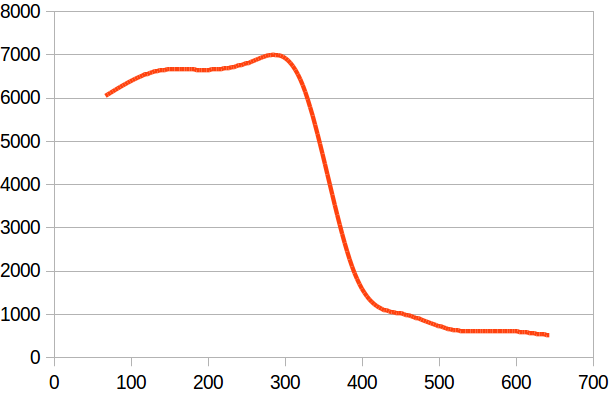
\includegraphics[width=4in]{images/SmallScale.png}
  \caption{TPS on our IBM x3650 system with 1 vCPU and 512KB vRAM. It changes from a memory bound application to an I/O bound application when the DB size approache the available RAM.}
  \label{smallIO}
  \end{center}
\end{figure}

We can use the TPS to show how the database performs at the application layer when external environment changes are made to the system.  Our tests will select Memory and I/O resources to monitor.  For measuring disk I/O it is a good to also collect virtual memory (in this case we are talking about OS virtual memory, not virtualization) as well as I/O data.  We selected to measure paging performance counters \ref{fig:memory} across all layers for the memory resource.  We selected disk read counters \ref{fig:io} as our data at all layers to measure interference from I/O. 

